\documentclass{beamer}

\usepackage[linesnumbered,ruled,french,onelanguage]{algorithm2e}
\usepackage{listings}

\usepackage[utf8]{inputenc}
\usepackage[T1]{fontenc}

\usetheme{CambridgeUS}

\setbeamertemplate{navigation symbols}{}% pour enlever les symboles de navigation en bas de chaque page
\setbeamertemplate{footline}[frame number]%pour changer le pied de page par un affichage des numér
 

\title{Corewar}
\date{26 Avril 2022}
\author{Alexander Camatchy \\ Alix Danvy \\ Mateo Delerue \\ Abdoulaye Fofana}
\institute{Université de Caen Normandie}

\begin{document}

\maketitle 

\begin{frame}
\tableofcontents
\end{frame}

\section{Corewar}
\begin{frame}
\frametitle{Introduction Corewar}
\begin{figure}
	\centering
	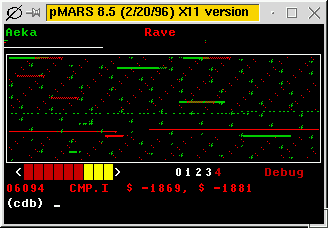
\includegraphics[width=0.7\textwidth]{images/PMars.png}
	\caption{pMars Interpreter}
\end{figure}
\end{frame}

\begin{frame}
	\frametitle{RedCode}
	\begin{table}[h!]
		\begin{center}
			\begin{tabular}{l|l}
				\textbf{Instruction} & \textbf{Action} \\
				\hline
				MOV A B & move A to B\\
				ADD A B & add A to B \\
				SUB A B & substract A from B\\
				JMP A B & jump to A\\
				JMZ A B & jump to A if B is zero\\
				JMN A B & jump to A if B is not zero\\
				CMP A B & if A equals B then skip the next instruction\\
				SLT A B & if A is less than B then skip the next instruction\\
				DJN A B & decrement B then if B is not zero jump to A\\
				SPL A B & create a new process at A\\
				DAT A B & the process dies\\
			\end{tabular}
		\end{center}
	\end{table}
\end{frame}

\begin{frame}[fragile]
	\frametitle{RedCode}
	\begin{table}[h!]
		\begin{center}
			\begin{tabular}{p{0.15\linewidth}|p{0.2\linewidth}|p{0.5\linewidth}}
				\textbf{Notation} & \textbf{Mode d'addressage} & \textbf{Action} \\
				\hline
				A & Direct & Accède à la case A relativement à la case courante\\
				\hline
				\#A & Octothorpe & Donne la valeur A\\
				\hline
				\symbol{64}A & Indirect & Accède à la case ayant l'addresse contenue dans la case A\\
				\hline
				<A & Pre-decremente & Décrémente la valeur contenue dans la case A puis accède à la case correspondant à cette addresse\\
				\hline
				>A & Pre-incremente & Incrémente la valeur cont
enue dans la case A puis accède à la case correspondant à cette addresse\\
			\end{tabular}
		\end{center}
	\end{table}
\end{frame}

\begin{frame}[containsverbatim]
\frametitle{RedCode}
\begin{figure}
\begin{lstlisting}
ca      equ 9
cb      equ -960

        mov 5, <-1
a       add @2, 3
        sub >ca+1, 10
        jmp aa, #ca
aa      jmz -9*-2, #+3
        jmn -a, @2
        cmp @-9, <8
aaa     slt 1, >0+2
        djn 325644521, a-1
        spl @34*31, @cb/2
\end{lstlisting}
\caption{Exemple de code source RedCode en norme ICWS-88}
\end{figure}
\end{frame}

\begin{frame}
\frametitle{Architecture}
\begin{figure}
	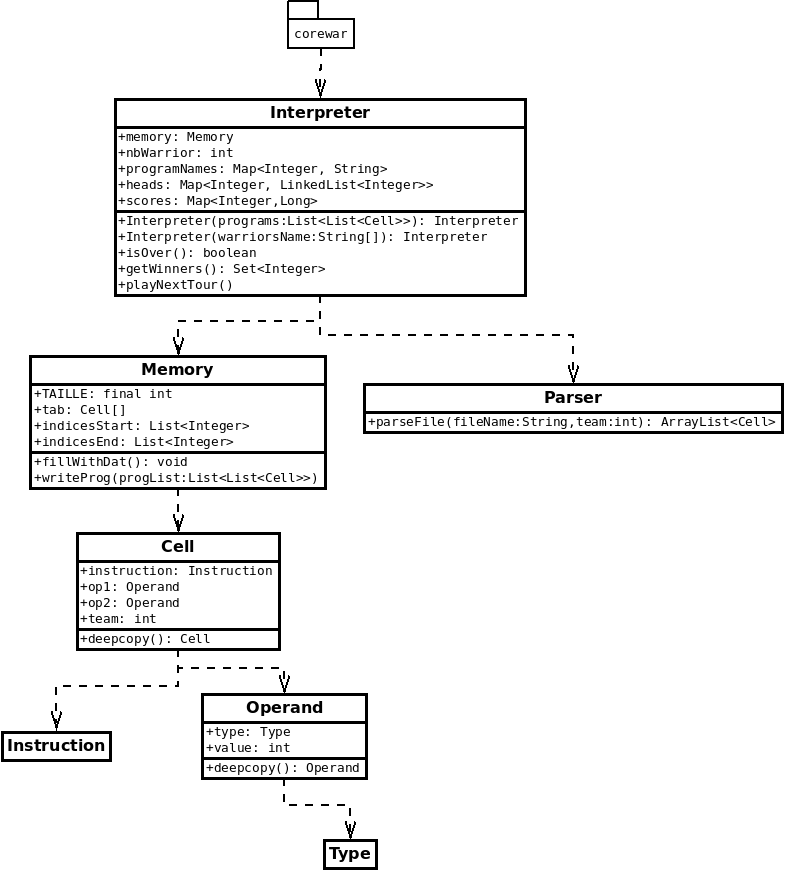
\includegraphics[height=0.7\textheight]{images/diagram-corewar.png}
	\caption{Diagramme de classe du projet}
\end{figure}
\end{frame}

\begin{frame}
\frametitle{Fonctionnement}
	\begin{algorithm}[H]
\DontPrintSemicolon
\SetKwData{args}{arguments}
$programs \gets Parser.parseFiles(args)$\;
$memory.writePrograms(programs)$\;
\While{$!interpreter.isOver()$}{
  \For{$program \in interpreter.programs$}{
    $head \gets program.popProcess()$\;
    $nextHead \gets interpreter.execute(memory.fetch(head))$\;
    \If(\tcp*[h]{Tête toujours en vie}){$nextHead != null$}{
      $program.pushProcess(nextHead)$\;
    }
  }
}
\caption{Pseudo-algorithme du déroulement d'une partie}
\end{algorithm}
\end{frame}

\section{Algorithme Génétique}
\subsection{Fonctionnement}
\begin{frame}
\frametitle{Algorithme Génétique}
\begin{figure}
	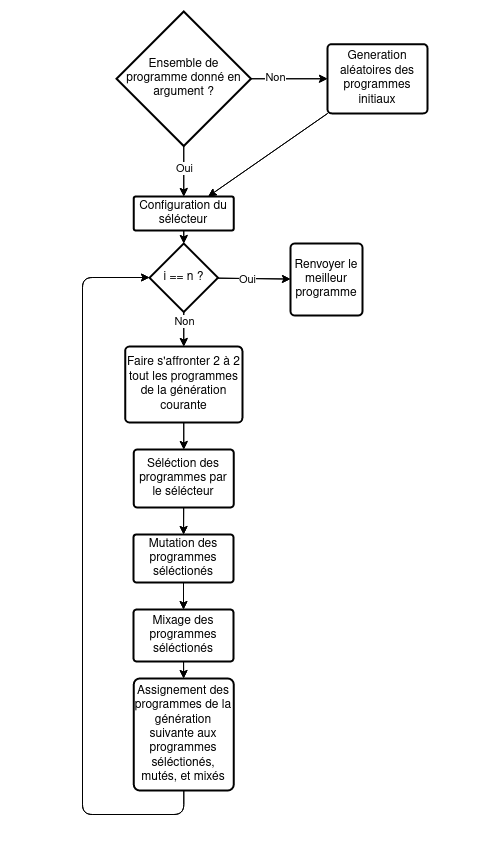
\includegraphics[height=0.8\textheight]{images/schema-algogen.png}
	\caption{Schéma du fonctionnement de l'algorithme génétique}
\end{figure}
\end{frame}

\begin{frame}
\frametitle{Architecture}
\begin{figure}
	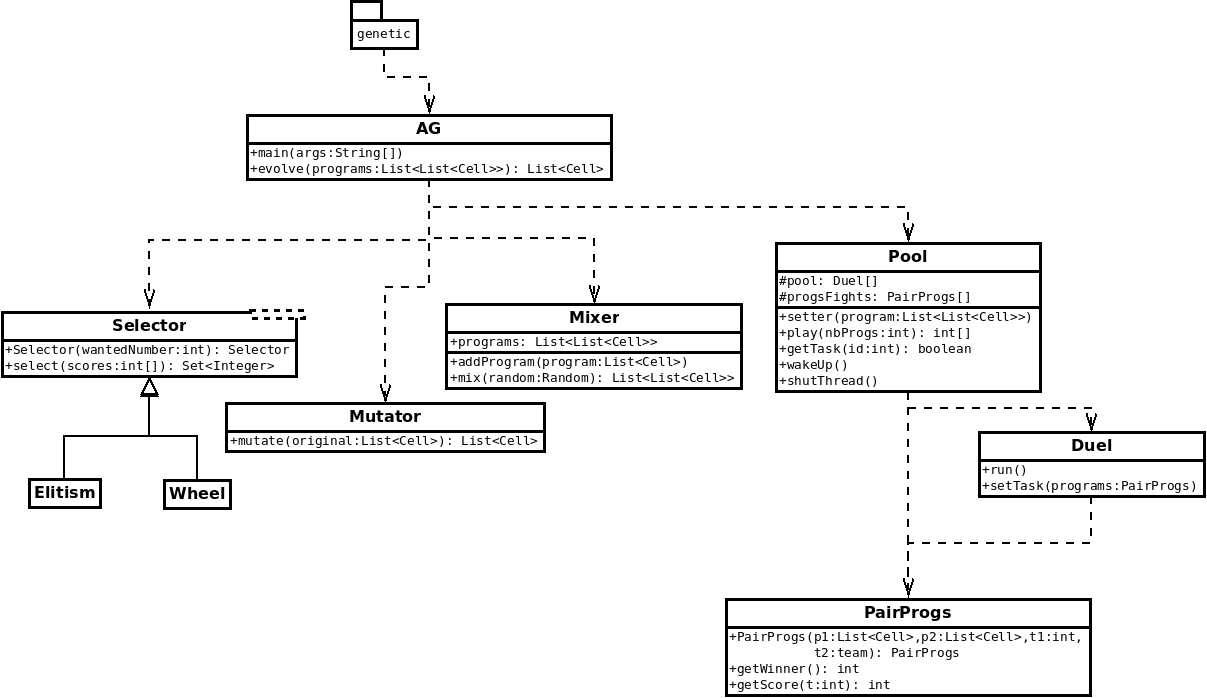
\includegraphics[height=0.7\textheight]{images/diagram-algogen.png}
	\caption{Diagramme de classe du package de l'algorithme génétique}
\end{figure}
\end{frame}

\subsection{Parrallélisme}
\begin{frame}
\frametitle{Parrallélisme}
\begin{block} {Pool}
	\begin{itemize}
		\item Initalisation:	\begin{itemize}
								\item Création des Threads (4 par défaut).
								\item Lancement des Threads.
							\end{itemize}
		\item Préparation:	\begin{itemize}
								\item Récupération des programmes à évaluer.
								\item Préparation des tâches pour les Threads.
							\end{itemize}
		\item Évaluation:	\begin{itemize}
								\item Réveil des Threads.
								\item Attente des Threads.
								\item Évaluation des résultats.
							\end{itemize}
		\item Fin: Arrêt des Threads. 
	\end{itemize}
\end{block} 
\end{frame}

\begin{frame}
\frametitle{Parrallélisme}
\begin{block} {Threads}
	\begin{itemize}
		\item Lancement: 
			\begin{itemize}
				\item Mise en attente.
				\item Attente d'un signal de la Pool.
				\item Demande de tâche à la Pool :	
					\begin{itemize}
						\item Tâche disponible: attribution et traitement, retour demande de tâche.
						\item Plus de tâche disponibles: retour mise en attente.								\end{itemize}
			\end{itemize}
		\item Fin: Arrêt du fonctionnement. 
	\end{itemize}
\end{block} 

\end{frame}


\subsection{Résultats}
\begin{frame}
\frametitle{Résultats}
\begin{columns}[c]
    \begin{column}{.45\textwidth}
    \begin{figure}
        \centering
        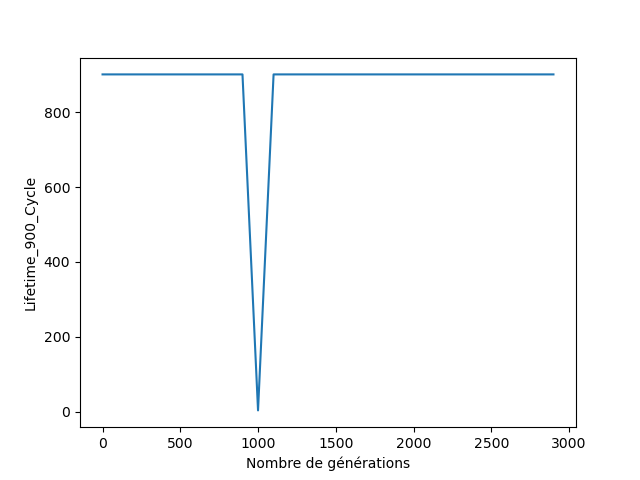
\includegraphics[width=1\textwidth]{images/Lifetime_900_Cycle.png}
        \caption{Best program lifetime over 900 cycle.}
    \end{figure}    
      
    \end{column}
    \begin{column}{.45\textwidth}
    \begin{figure}
        \centering
        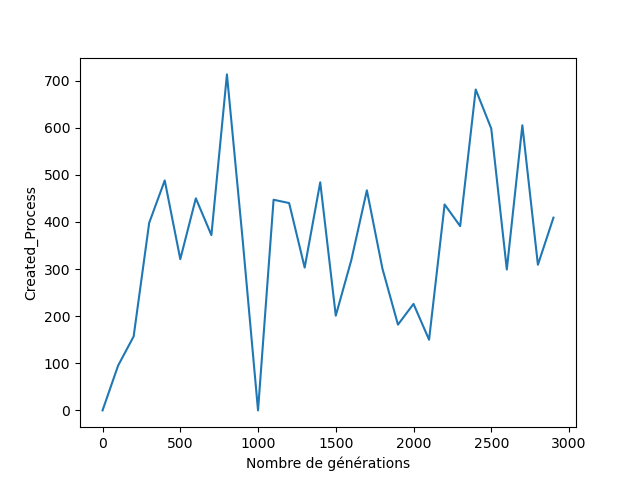
\includegraphics[width=1\textwidth]{images/Created_Process.png}
        \caption{Number of created process over 900 cycle.}
    \end{figure}
    \end{column}
\end{columns}

\end{frame}

\begin{frame}
\frametitle{Résultats}
\begin{columns}[c]
    \begin{column}{.45\textwidth}
    \begin{figure}
        \centering
        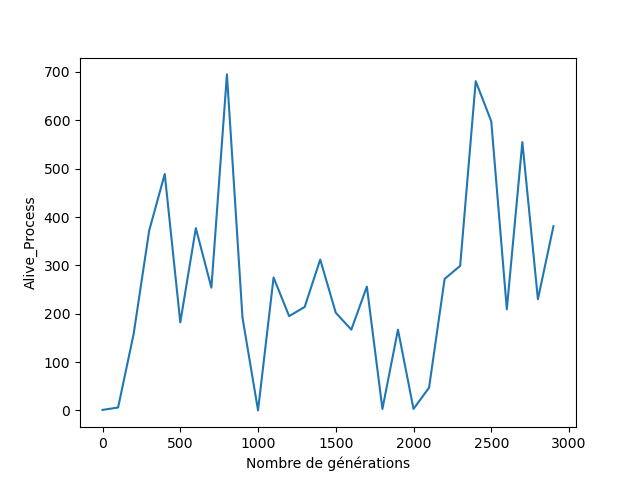
\includegraphics[width=1\textwidth]{images/Alive_Process.png}
        \caption{Number of alive process after 900 cycle.}
    \end{figure}    
      
    \end{column}
    \begin{column}{.45\textwidth}
    \begin{figure}
        \centering
        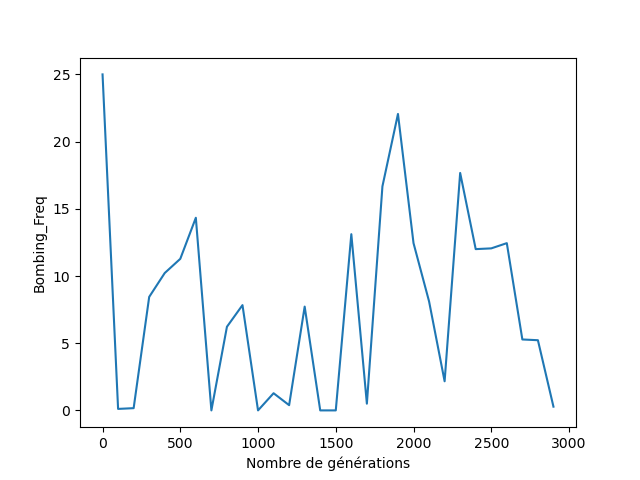
\includegraphics[width=1\textwidth]{images/Bombing_Freq.png}
        \caption{Bombing frequence of the program (~ average bombing over 50 cycle).}
    \end{figure}
    \end{column}
\end{columns}

\end{frame}

\begin{frame}
\frametitle{Résultats}
\begin{columns}[c]
    \begin{column}{.45\textwidth}
    \begin{figure}
        \centering
        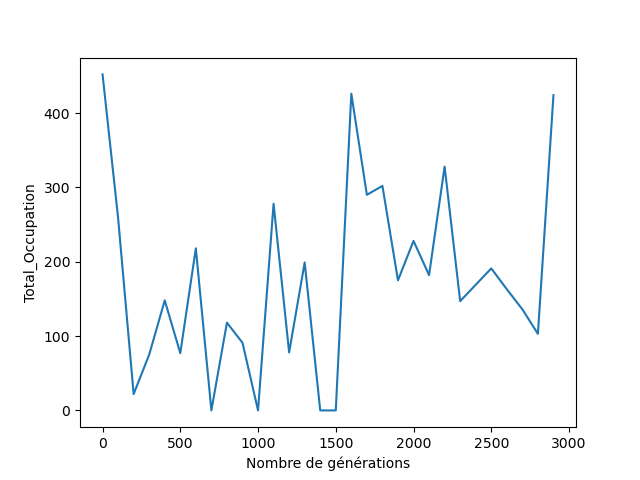
\includegraphics[width=1\textwidth]{images/Total_Occupation.png}
        \caption{Number of written cell over 900 cycle.}
    \end{figure}    
      
    \end{column}
    \begin{column}{.45\textwidth}
    \begin{figure}
        \centering
        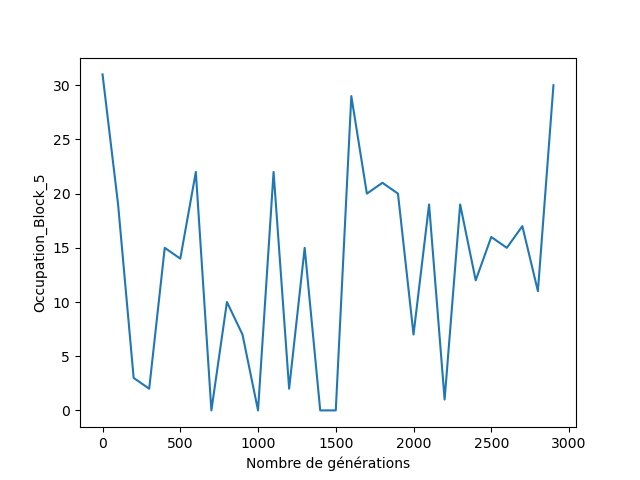
\includegraphics[width=1\textwidth]{images/Occupation_Block_5.png}
        \caption{Number of block of five cell that have at least one cell written by the program on over 900 cycle.}
    \end{figure}
    \end{column}
\end{columns}

\end{frame}

\section{Interface Graphique}
\begin{frame}
\frametitle{Interface Graphique}
\begin{figure}
	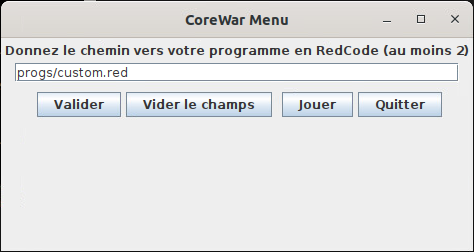
\includegraphics[height=0.4\textheight]{images/mainMenu.png}
	\caption{Menu principal où l'on choisit les programmes}
\end{figure}
\begin{figure}
	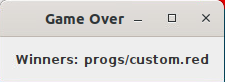
\includegraphics[height=0.2\textheight]{images/gameOver.png}
	\caption{Pop-up Qui affiche le programme gagnant}
\end{figure}
\end{frame}
		
\begin{frame}
\frametitle{Interface Graphique}
\begin{figure}
	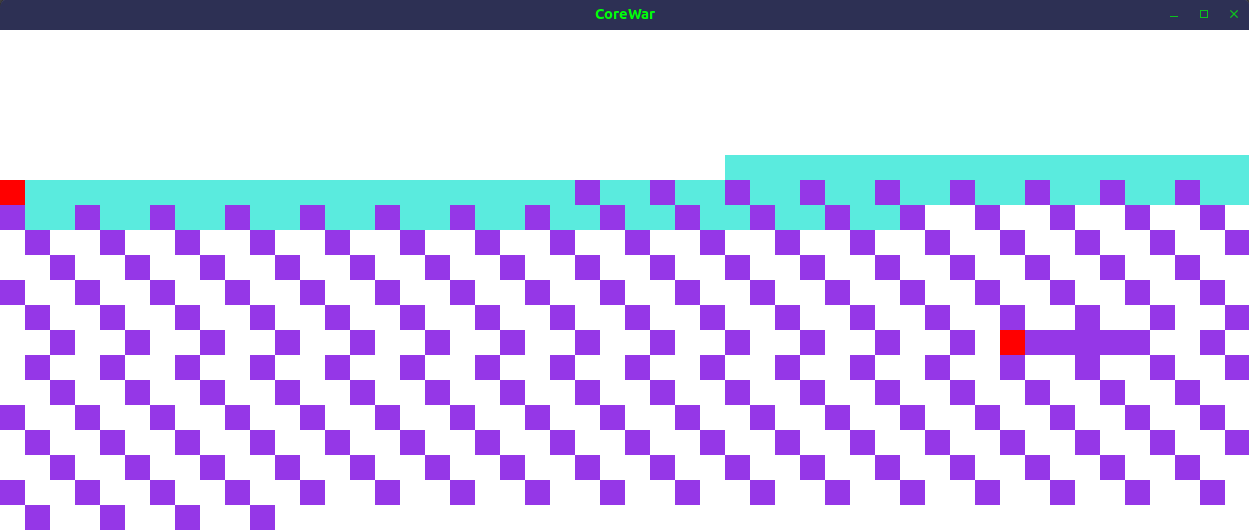
\includegraphics[height=0.4\textheight]{images/jeu.png}
	\caption{Jeu principal}
\end{figure}
\end{frame}

\section{Conclusion}
\begin{frame}
\frametitle{Conclusion}
\begin{itemize}
	\item Objectifs atteints.
	\item Ce qu'on a appris.
	\item Pistes d'améliorations.
	\item Avenir du projet.
	
\end{itemize}
\end{frame}

\end{document}
